% ------------------------------------------------------------------------------
% TYPO3 CMS 8.4 - What's New - Chapter "Deprecated Functions" (Italian Version)
%
% @author	Michael Schams <schams.net>
% @license	Creative Commons BY-NC-SA 3.0
% @link		http://typo3.org/download/release-notes/whats-new/
% @language	English
% ------------------------------------------------------------------------------
% LTXE-CHAPTER-UID:		3f842373-9262b8d3-f9c8de76-cf29ce17
% LTXE-CHAPTER-NAME:	Deprecated Functions
% ------------------------------------------------------------------------------

\section{Funzionalità deprecate/rimosse}
\begin{frame}[fragile]
	\frametitle{Funzionalità deprecate/rimosse}

	\begin{center}\huge{Capitolo 5:}\end{center}
	\begin{center}\huge{\color{typo3darkgrey}\textbf{Funzionalità deprecate/rimosse}}\end{center}

\end{frame}

% ------------------------------------------------------------------------------
% LTXE-SLIDE-START
% LTXE-SLIDE-UID:		3f7f42ce-97d75ed4-7122411f-f1c9d0e2
% LTXE-SLIDE-ORIGIN:	cf7400eb-0f683329-f6c51cbf-dfd192d9 English
% LTXE-SLIDE-TITLE:		#77630: Remove wizard icons
% ------------------------------------------------------------------------------
\begin{frame}[fragile]
	\frametitle{Funzionalità deprecate/rimosse}
	\framesubtitle{Icone nello Wizard rimosse}

	\begin{itemize}

		\item Le seguenti icone sono state rimosse dallo FormFieldWizard:

			\begin{itemize}
				\item \texttt{wizard\_add.gif}
				\item \texttt{wizard\_edit.gif}
				\item \texttt{wizard\_link.gif}
				\item \texttt{wizard\_list.gif}
				\item \texttt{wizard\_rte.gif}
				\item \texttt{wizard\_table.gif}
			\end{itemize}

	\end{itemize}

	\begin{figure}
		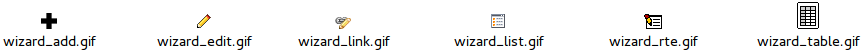
\includegraphics[width=0.95\linewidth]{DeprecatedRemovedFunctions/77630.png}
	\end{figure}

\end{frame}

% ------------------------------------------------------------------------------
% LTXE-SLIDE-START
% LTXE-SLIDE-UID:		4586b1e4-1eb786cf-31c6544d-56467a02
% LTXE-SLIDE-ORIGIN:	d5ced5e7-04dffe16-b8ec9f2c-712020cd English
% LTXE-SLIDE-TITLE:		#77693: Remove/Move Icons from EXT:t3skin
% ------------------------------------------------------------------------------

\begin{frame}[fragile]
	\frametitle{Funzionalità deprecate/rimosse}
	\framesubtitle{Icone del \texttt{EXT:t3skin}}

	\begin{itemize}

		\item Le icone di \texttt{EXT:t3skin} sono state rimosse o spostate
		\item \textbf{Rimosse:}

			\begin{itemize}
				\item \smaller\texttt{typo3/sysext/t3skin/icons/gfx/error.png}
				\item \texttt{typo3/sysext/t3skin/icons/gfx/i/\_icon\_ftp.gif}
				\item \texttt{typo3/sysext/t3skin/icons/gfx/information.png}
				\item \texttt{typo3/sysext/t3skin/icons/gfx/notice.png}
				\item \texttt{typo3/sysext/t3skin/icons/gfx/warning.png}
			\end{itemize}

		\item \textbf{Spostate:}

			\begin{itemize}
				\item \smaller\texttt{typo3/sysext/t3skin/icons/gfx/icon\_fatalerror.gif}
				\item \texttt{typo3/sysext/t3skin/images/icons/status/status-edit-read-only.png}
				\item \texttt{typo3/sysext/t3skin/images/icons/status/warning-in-use.png}
				\item \texttt{typo3/sysext/t3skin/images/icons/status/warning-lock.png}
				\item \texttt{typo3/sysext/t3skin/images/icons/status/status-reference-hard.png}
				\item \texttt{typo3/sysext/t3skin/images/icons/status/status-reference-soft.png}
			\end{itemize}

	\end{itemize}

\end{frame}

% ------------------------------------------------------------------------------
% LTXE-SLIDE-START
% LTXE-SLIDE-UID:		cf08f76b-1c4294e4-1559e5b5-3a6790c3
% LTXE-SLIDE-ORIGIN:	7848f0b0-d687b337-f7638646-680dc819 English
% LTXE-SLIDE-TITLE:		Obsolete page tree and click menu settings removed
% ------------------------------------------------------------------------------

\begin{frame}[fragile]
	\frametitle{Funzionalità deprecate/rimosse}
	\framesubtitle{Albero delle pagine e funzionalità del "click menu"}

	\begin{itemize}

		\item Le funzionalità obsolete dell'albero delle pagine e del "click menu" sono state rimosse
		\item \textbf{Proprietà}:

		\begin{itemize}
			\item \texttt{FileSystemNavigationFrameController->doHighlight}
			\item \texttt{ClickMenu->leftIcons}
		\end{itemize}

		\item \textbf{Impostazioni TypoScript}:

		\begin{itemize}
			\item \texttt{options.pageTree.disableTitleHighlight}
			\item \texttt{options.contextMenu.options.leftIcons}
		\end{itemize}

	\end{itemize}

\end{frame}

% ------------------------------------------------------------------------------
% LTXE-SLIDE-START
% LTXE-SLIDE-UID:		1f2672eb-e3ff9d62-9f34032b-7dfd7a42
% LTXE-SLIDE-ORIGIN:	aad23a73-7b046eaf-fb4bb862-2f88ef71 English
% LTXE-SLIDE-TITLE:		ExtensionManagementUtility::extRelPath()
% LTXE-SLIDE-REFERENCE:	#78193: ExtensionManagementUtility::extRelPath() deprecated
% ------------------------------------------------------------------------------

\begin{frame}[fragile]
	\frametitle{Funzionalità deprecate/rimosse}
	\framesubtitle{ExtensionManagementUtility::extRelPath()}

	\begin{itemize}

		\item Il metodo \texttt{ExtensionManagementUtility::extRelPath()} è stato impostato come deprecato
		\item Questo metodo era usato per ottenere il path relativo allo script corrente
		\item Sono disponibili metodi alternativi:

			\begin{itemize}
				\item \texttt{ExtensionManagementUtility::extPath()}\newline
					(per ottenere il percorso completo di un estensione)
				\item \texttt{ExtensionManagementUtility::siteRelPath()}\newline
					(per ottenere il percorso relativo di un estensione rispetto a \texttt{PATH\_site}
				\item \texttt{GeneralUtility::getFileAbsFileName()}\newline
					(per ottenere il percorso prefissato di EXT:myextension
				\item \texttt{PathUtility::getAbsoluteWebPath()}\newline
					(per ottenere il percorso assoluto prefissato per una cartella web)
			\end{itemize}

	\end{itemize}

\end{frame}

% ------------------------------------------------------------------------------
% LTXE-SLIDE-START
% LTXE-SLIDE-UID:		9a840582-dee8434d-789ae0d0-e93b01ff
% LTXE-SLIDE-ORIGIN:	43a5eaf5-8945a8d5-ac27d4ea-24ffc8e3 English
% LTXE-SLIDE-TITLE:		Miscellaneous (1) (#75363)
% LTXE-SLIDE-REFERENCE:	#75363: Deprecate FormResultCompiler->JStop()
% LTXE-SLIDE-REFERENCE:	#75637: Deprecate optional parameters of RecyclerUtility::getRecordPath()
% ------------------------------------------------------------------------------

\begin{frame}[fragile]
	\frametitle{Funzionalità deprecate/rimosse}
	\framesubtitle{Varie (1)}

	\begin{itemize}
		\item Il metodo \texttt{FormResultCompiler->JStop()} è stato rinominato con \texttt{addCssFiles()}.
			Il vecchio metodo è ancora presente come deprecato e sarà rimosso in TYPO3 v9.

		\item Il metodo \texttt{ClickMenu::DB\_editPageProperties()} è stato marcato come deprecato

		\item I seguenti argomenti del metodo \texttt{RecyclerUtility::getRecordPath()} sono stati marcati come deprecati:

			\begin{itemize}
				\item \texttt{\$clause}
				\item \texttt{\$titleLimit}
				\item \texttt{\$fullTitleLimit}
			\end{itemize}

	\end{itemize}

\end{frame}

% ------------------------------------------------------------------------------
% LTXE-SLIDE-START
% LTXE-SLIDE-UID:		d2e07b98-97f8adbc-d2442864-e97161fd
% LTXE-SLIDE-ORIGIN:	0745e3f3-83db03d7-ac24e92a-300391ba English
% LTXE-SLIDE-TITLE:		Miscellaneous (2) (#77783 and #77826)
% LTXE-SLIDE-REFERENCE:	#77783: Unused ExtJS JavaScript libraries removed
% LTXE-SLIDE-REFERENCE:	#77826: RTEHtmlArea Spellchecker eID removed
% ------------------------------------------------------------------------------

\begin{frame}[fragile]
	\frametitle{Funzionalità deprecate/rimosse}
	\framesubtitle{Varie (2)}

	\begin{itemize}

		\item Le seguenti librerie ExtJS JavaScript non utilizzate sono state rimosse:

			\begin{itemize}
				\item \texttt{app.SearchField}
				\item \texttt{grid.RowExpander}
				\item \texttt{ux.FitToParent}
			\end{itemize}

		\item Il RTEHtmlArea eID (\texttt{rtehtmlarea\_spellchecker}), per l'utilizzo
			del correttore automatico, è stato rimosso e l'entry point per le richieste HTTP di
			\texttt{SpellCheckingController->main} è stato marcato come deprecato

		\item Il formato \texttt{DateTime::ISO8601} è incompatibile con ISO-8601,
			ma è stato lasciato per ragioni di compatibilità all'indietro.
			Le costanti \texttt{DateTime::ATOM} o \texttt{DATE\_ATOM} vanno usate invece.

	\end{itemize}

\end{frame}

% ------------------------------------------------------------------------------
% LTXE-SLIDE-START
% LTXE-SLIDE-UID:		2642b79e-deec9133-18614e0f-57d0c77f
% LTXE-SLIDE-ORIGIN:	0745e3f3-83db03d7-ac24e92a-300391ba English
% LTXE-SLIDE-TITLE:		Miscellaneous (3) (#77839, #78096 and #78222)
% LTXE-SLIDE-REFERENCE:	#77839: TYPO3/CMS/Core/QueryGenerator
% LTXE-SLIDE-REFERENCE:	#78096: Deprecate PageLayoutView::getResult with mysqli_result objects
% LTXE-SLIDE-REFERENCE:	#78222: Late generation of autoload information is deprecated
% ------------------------------------------------------------------------------

\begin{frame}[fragile]
	\frametitle{Funzionalità deprecate/rimosse}
	\framesubtitle{Varie (3)}

	\begin{itemize}

		\item Il modulo AMD \texttt{TYPO3/CMS/Core/QueryGenerator} è stato spostato in EXT:lowlevel\newline
			\small
				(e rinominato in \texttt{TYPO3/CMS/Lowlevel/QueryGenerator})
			\normalsize

		\item Il metodo \texttt{PageLayoutView::getResult()} è stato marcato come deprecato
			nell'uso dell'oggetto \texttt{mysqli\_result} come primo parametro

		\item Se TYPO3 non è in modalità composer, veniva utilizzato automaticamente il dump delle classi delle estensioni
			nel caricamento delle informazioni nella fase di bootstrap. Questo comportamento è ora deprecato.
	\end{itemize}

\end{frame}

% ------------------------------------------------------------------------------
